\section{Chapter Overview}
The first step in creating an \ac{FPGA} based network of \ac{ADPLL}s is the design of the \ac{ADPLL} itself, which will be addressed in this chapter. The nature of an \ac{FPGA} necessitates a number of compromises in the design of a given block which limits transferability to \ac{ASIC} designs. In this chapter the potential designs for each individual block, or module, investigated will be explained and the case for their selection in an \ac{FPGA} based \ac{ADPLL} made. A number of blocks have implement purely digital circuitry and as such can be transferred in their entirety from an \ac{FPGA} and vice versa. However, those that will be used to emulate mixed-signal circuitry, such as the \ac{DCO} and \ac{PFD}, will be examined in greater detail.
\begin{figure}[h] %TODO redo this image
	\centering
	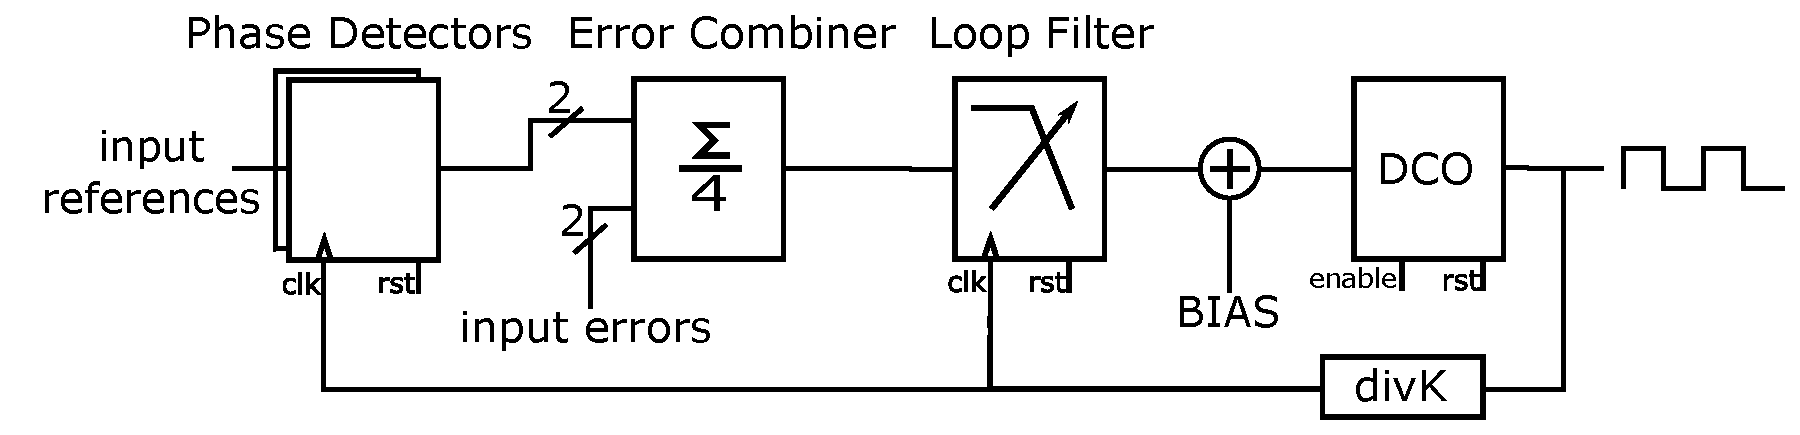
\includegraphics[width=\textwidth]{../network_adpll}
	\caption{\ac{ADPLL} designed for use in a Cartesian grid network.}
	\label{fig:dist_adpll}
\end{figure}

\section{Digitally Controlled Oscillators}
The choices made in the design of the \ac{DCO} have the greatest impact on the effectiveness of the overall platform and which use cases the \ac{ADPLL} containing it are suitable for, as the key performance benchmarks are all done using the waveform this block generates. This project will address three distinct designs of \ac{ADPLL}s suitable for implementation on an FPGA, two derived from the clocks generated by the \ac{FPGA}s own distribution network and one generated independently of this clock, using a chain of inverters. These are not the only ways in which an oscillator could be synthesised on an \ac{FPGA}, however other designs were deemed to be unsuitable for extensible and portable implementations.

A prime example of this is the use of Xilinx proprietary \texttt{IODELAY} blocks to create an oscillator, as detailed in Xilinx Application Note XAPP872 \cite{iodelay}. The key idea here is that the bulk of the period is made up by the propagation time through one of the \texttt{IODELAY} blocks, which can be set at implementation time. This is combined with a section of an inverter chain, and a multiplexer used modify the length of this segment, the output of which is fed back into the \texttt{IODELAY} block. This method was discarded as the number of \texttt{IODELAY} blocks is very limited, so expanding to a larger network would be impossible, and they are all located around the edge of the chip, not suited to the construction of a Cartesian grid.

The main issue with the creation of \ac{DCO}s on an \ac{FPGA} is the inability to create mixed-signal circuits, such as those that would be intended for use on an \ac{ASIC}. As such the \ac{FPGA} based oscillator must emulate the behaviour of a mixed-signal circuit in some way.

\subsection{\acs{FPGA} Driven, Linear Period \acs{DCO}}
\begin{figure}[h]
	\centering
	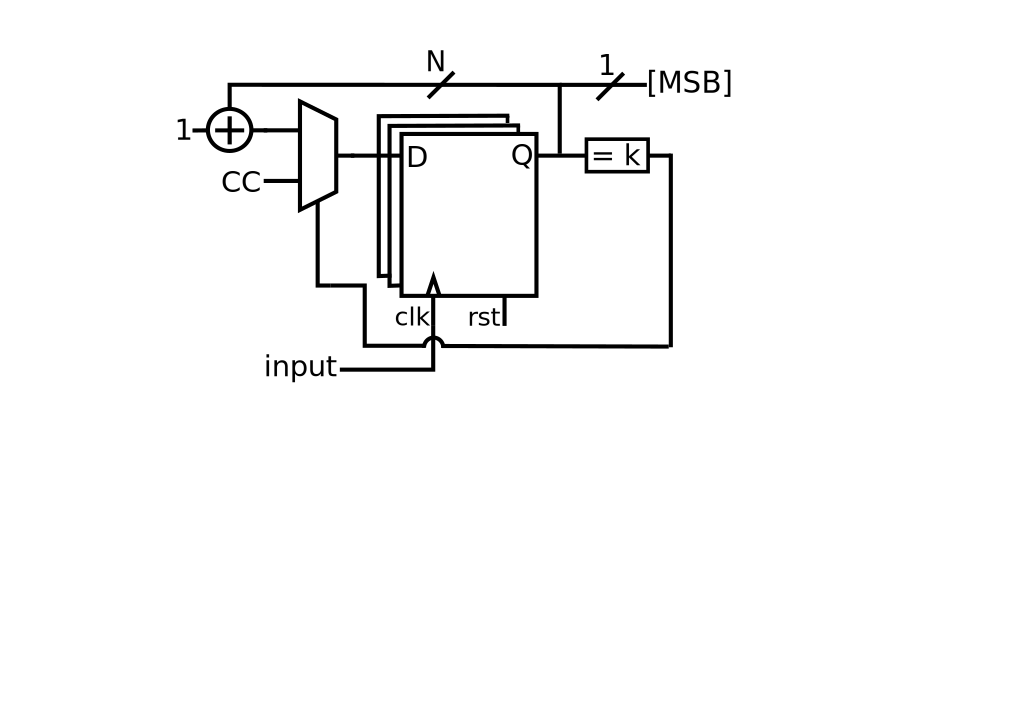
\includegraphics[width=0.6\textwidth]{../osc1}
	\caption{\acs{FPGA} driven, linear period \acs{DCO} \ac{RTL} Diagram.}
	\label{fig:osc1}
\end{figure}
The first design of \ac{DCO} to be examined is of the type used by Zianbetov in his \ac{ADPLL} network test bed and relies on a counter driven by the clock manager on the \ac{FPGA} \cite{zianbetov2013phd}. At each event on the \ac{FPGA} provided clock a counter is incremented, overflowing upon increment past the maximum possible value. The \ac{MSB} of this counter forms the waveform generated by this oscillator, the period of which is controlled through an adjustable value that is loaded into the counter once overflow is reached, and forms the starting points for the counter. The period of oscillation is given by:
\begin{equation}
	T_{osc} = \big(2^{width} -~(BIAS+CC)~\big)\times T_{FPGA}
\end{equation}
where $T_{FPGA}$ is the clock period of the \ac{FPGA}, $CC$ is the control code input, $BIAS$ centres the oscillator in the middle of the tuning range in the event that the control code is zero and $width$ is the width of the counter used. As the only variable here is the control code, period step of this design is $T_{FPGA}$, thereby providing period linearity with respect to the control code. This is the key advantage of this design, as most \ac{ASIC} implementations of a \ac{DCO} are also linear in period. The other main reason to choose this design is that its \ac{FPGA} clocked nature allows for exact control over the frequency of operation, and the number of tunable parameters make it possible to configure multiple ways to achieve the same frequencies of operation. Combined these attributes make it very easy to create an oscillator that emulates the behaviour of a design intended for an \ac{ASIC}, however, at a greatly reduced frequency. This restriction on the frequency of operation arises out of the period step size, which in order to obtain a good resolution must be orders of magnitude smaller than the intended period to be generated. As the output waveform is taken from the counter's \ac{MSB}, the reload value of the counter must never go beyond $2^{width-1}$, as otherwise the output waveform will become a constant 1. As the reload value varies the low time of the \ac{MSB}, if the desired output waveform is a square wave this design will not be suitable.

In being \ac{FPGA} clocked this design has pseudo-deterministic characteristics, with each period step being almost identical across oscillators and over the entire tuning range, unlike an \ac{ASIC} where process variation will impact the layout of a high frequency oscillator. The only variation in this design will come, ironically, from jitter or skew in the \ac{FPGA}'s clock distribution network, which as the frequencies will typically be in the low hundreds of MHz is very minor. In the case of the Xilinx \acl{Nexys} this is at most 100 picoseconds, or 0.05\% of the period of an intended output clock at 5 MHz. To put this value into perspective, on this board the minimum value of $T_{FPGA}$ that could be used to drive this oscillator is 3.87 nanoseconds, 1.935\% of the period.

The resulting \ac{DCO} is best suited to applications that do not seek to gain a better understanding of oscillator performance, but rather those focused on validating the entirely digital blocks in the system, the role in which Zianbetov and Shan used this type of oscillator \cite{zianbetov2013phd,shan2014phd}.

\subsection{\acs{FPGA} Driven, Linear Frequency \acs{DCO}}
\begin{figure}[h]
	\centering
	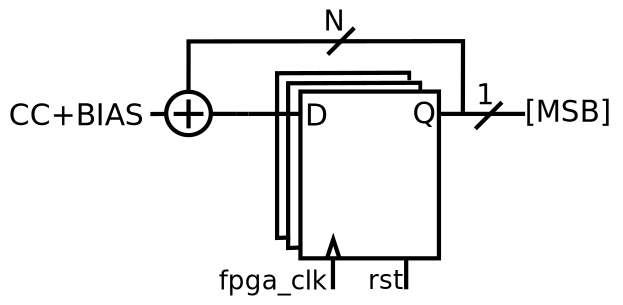
\includegraphics[width=0.6\textwidth]{../osc2}
	\caption{\acs{FPGA} driven, linear frequency \acs{DCO} \ac{RTL} Diagram.}
	\label{fig:osc2}
\end{figure}
The second \ac{FPGA} clocked oscillator is similar in most attributes to the above design but eschews period linearity for frequency linearity. Again the overflow property of a counter is used with the counter's \ac{MSB} as output of the block, however, this time it forms a square wave. Rather than setting the reload value of the counter, instead the increment is adjusted depending on the control code, thus requiring $\frac{2^N}{BIAS+CC}$ increments to overflow. Accordingly the frequency of operation is set by:
\begin{equation}
	f_{osc} = f_{FPGA}\times\frac{BIAS+CC}{2^{width}}
\end{equation}
Here the control code $CC$ and bias are added to the value stored in the accumulator at each event of the \ac{FPGA}, clock until overflow is reached. This occurs at $2^{width}$ where, as before, $width$ is the bit width of the counter, thus valuing each control code increment at $\frac{f_{FPGA}}{2^{width}}$ Hz. As with the previous design, this oscillator is better suited to frequencies where the output of the \ac{DCO} is orders of magnitude lower than the clock signal driving it, as this ensures that the incremental change due to the control code remains a small fraction of the period.

This design is just as configurable as its linear-in-period counterpart, and well suited to the low frequency emulation of \ac{ASIC} based oscillators that are themselves linear in frequency. In sharing the \ac{FPGA} as a clock source again the pseudo-deterministic characteristics return, once more meaning this oscillator is better used for testing, simulating or verifying other blocks in the system.

\subsection{Ring Oscillator}
The best approximation of the non-idealities of an \ac{ASIC} \ac{DCO} implementation can be obtained using a \ac{RO}, also know as an inverter ring, as the \ac{DCO}. In an \ac{ASIC} an \ac{RO} is constructed by connecting a number of NOT gates back in a chain, with the output of the last NOT gate fed input the input of the first. As NOT gates are not available on an \ac{FPGA}, they are replaced by inverter primitives. The inverter ring is an inherently unstable circuit that leverages the propagation delay through an odd number of inverters to create a waveform that, when viewed at a fixed position, is a square wave. 
\begin{figure}[h]
	\centering
	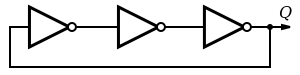
\includegraphics[width=0.4\textwidth]{../RO-wiki}
	\caption[Basic ring oscillator \ac{RTL} diagram]{Basic ring oscillator \ac{RTL} diagram \cite{ro_wiki}.}
	\label{fig:ro_wiki}
\end{figure}

The output value of the inverter at the end of the chain changes a non-zero amount of time after the input to the first element is set. It can be trivially shown that if the number of inverters is odd, this will be the inverse of the value initially applied to the first element. This sets in motion an oscillation, the period of which is governed by the number of inverters in the chain. The formula to calculate the oscillator's period is simple:
\begin{equation}
	T_{osc} = 2\times \tau_{inv} \times N
\end{equation}
Here, $\tau_{inv}$ is the propagation time through one inverter, $N$ is the number of inverters in the chain and the multiple of two arises from the necessity to invert twice to produce a square wave.

The main advantage of this type of oscillator stems from its similarity to that used on an \ac{ASIC} which leads to many non-idealities carrying over from the truly mixed-signal implementation. Rather than being just a tool to validate that other modules, the performance of this oscillator can be analysed more deeply as well as the performance of networks containing it. Koskin \textit{et al} used such a design to test theories proposed regarding the synchronisation of oscillators during his PhD using this type of oscillator implemented on an \ac{FPGA} \cite{koskin2019phd,theboys2019}.

While it is advantageous for the purposes of analysis that this design is affected by variation in temperature, implementation and other non-idealities this brings with it challenges not present in a true mixed-signal design. In a design intended for an \ac{ASIC} the design has near total control over the placement of circuit elements, however, the \ac{FPGA} based counterpart control is available over just the area in which the oscillator may lie, and the \ac{EDA} is responsible for the exact placement. Unlike the \ac{ASIC} implementation, in which the propagation delay through each element of the ring is well bounded, the lack of control over placement means that the propagation time through each inverter is not well bounded and may vary wildly. This makes it time consuming to ensure that the frequency tuning ranges of each oscillator match that desired, and use of this oscillator less straight-forward than that of the previous two designs.

\section{Frequency Divider}
Many \ac{PLL}s, be they digital or analogue, incorporate a frequency divider in the feedback path so that comparison can be made with a reference operating at a lower frequency. This is a feature that is advantageous for \ac{ADPLL} networks, as comparison using this divided clock allows the synchronisation signal sent between modules to be of a frequency orders of magnitude lower than that of the clock distribution network and thus require circuitry that consumes significantly less energy. This division can be obtained trivially on an \ac{FPGA} by a number of means, of which this thesis will mention just two. The first of these methods allows for integer division, by inverting a signal each time a counter reaches a certain value, $k$. When this condition is true the value stored in the counter is also reset to zero, thus implementing division of the generated clock frequency by $2k$.
\begin{figure}[h]%
	\centering
	\subfloat[Divider 1]{{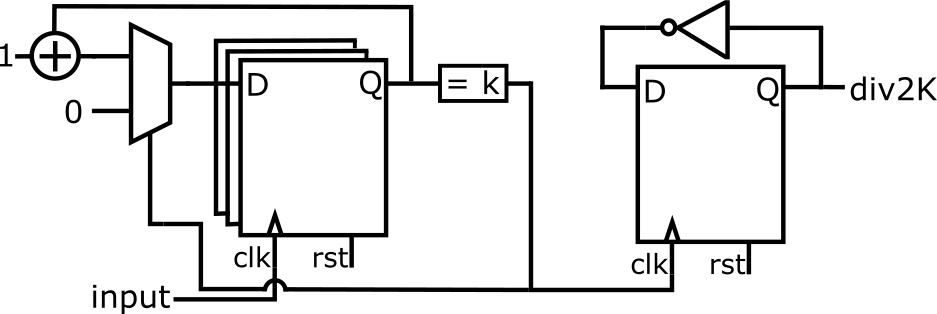
\includegraphics[width=0.6\textwidth]{../divider1} }}\\
	\subfloat[Divider 2]{{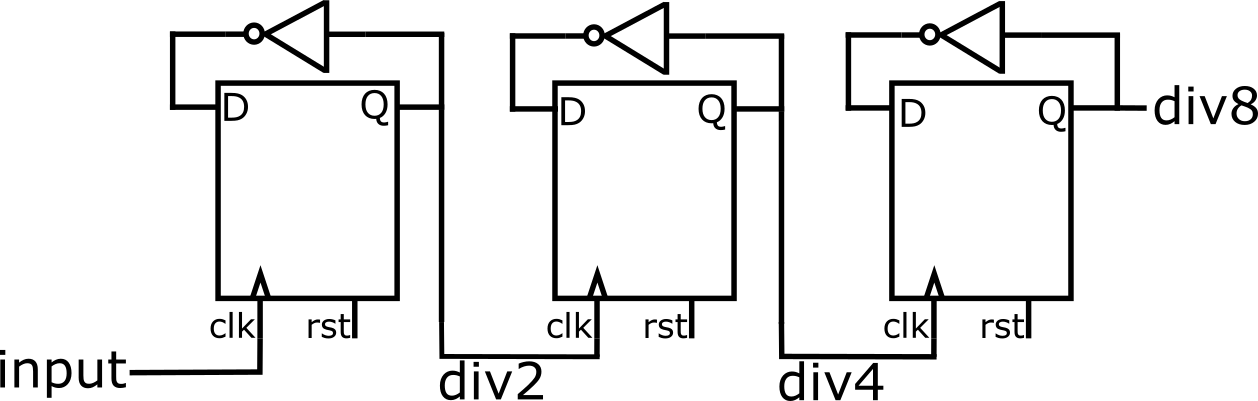
\includegraphics[width=0.6\textwidth]{../divider2} }}%
	\caption{Frequency divider \ac{RTL} diagrams.}
	\label{fig:divs}
\end{figure}
By limiting to division by powers of two, the divider can be simplified with the removal of any comparison logic. One flip-flop and an inverter are required per power of two. As in Figure \ref{fig:divider_2}, the inverted $\overline{Q}$ output of each flip-flop is inverted and connected to the $D$ input, with the non-inverted $Q$ of the previous flip-flop acting as the clock. The first flip-flop in the chain is clocked by the \ac{DCO} output. 

\section{Phase Detector}

\section{Error Combiner}
In a regular \ac{ADPLL} an error combining circuit is not required as there is never more than one reference signal, and as such the input of this block would be equivalent to the output. However in an \ac{ADPLL} network multiple reference signals are required, one for each neighbour, thus requiring some method to combine. Simply averaging these signals was not found to be viable by Pratt and Nyugen in their original paper for analogue systems, however, the work of Javidan \textit{et al}, showed that in a digital system this method will not result in mode locking, provided start-up is performed uni-directionally \cite{javidan2011all}.

Accordingly, any intended error combiner design implementing an average should also be reconfigurable, so that it satisfies the reconfigurability constraint. Given this is a digital system the most straightforward way to implement this is as a weighted sum, followed by a division. The final \ac{ADPLL} network will be laid out in a Cartesian grid so a maximum of four values will possibly be combined, with only the non-corner edge nodes having a number of neighbours that is not a power of two.
The simplest, and most processing time efficient, method of calculating the weighted sum restricts the weights to powers of two, as this permits their implementation as a left bit shift which is trivially achieved in hardware by a part select.
Similarly this reasoning can be expanded to the division, where the complicated division by three for a non-corner edge node is instead replaced by division by four. This means the division is implemented identically by all error combiners in the network, and implemented trivially by a right shift of two bits.%TODO ask pierre re 3 div 4

\section{Loop Filter}